\documentclass{article}

\usepackage{amsmath,amsfonts,amsthm}
\usepackage{graphicx}

\setlength\parindent{0pt} 
\newcommand{\horrule}[1]{\rule{\linewidth}{#1}}

\title{	
\normalfont \normalsize 
\textsc{Cornell University, INFO/CS 4740: Introduction to Natural Language Processing, Spring 2015} \\
\horrule{0.5pt} \\[0.4cm]
\huge PA 2: Question Answering \\ 
\horrule{2pt} \\[0.5cm]
}
\author{Sofonias Assefa (saa237), La Vesha Parker (ldp47)}
\date{\normalsize\today}
\begin{document}

\maketitle

\section{Description of QA System}
\subsection*{Overview}
\begin{figure}[h]
    \centering
    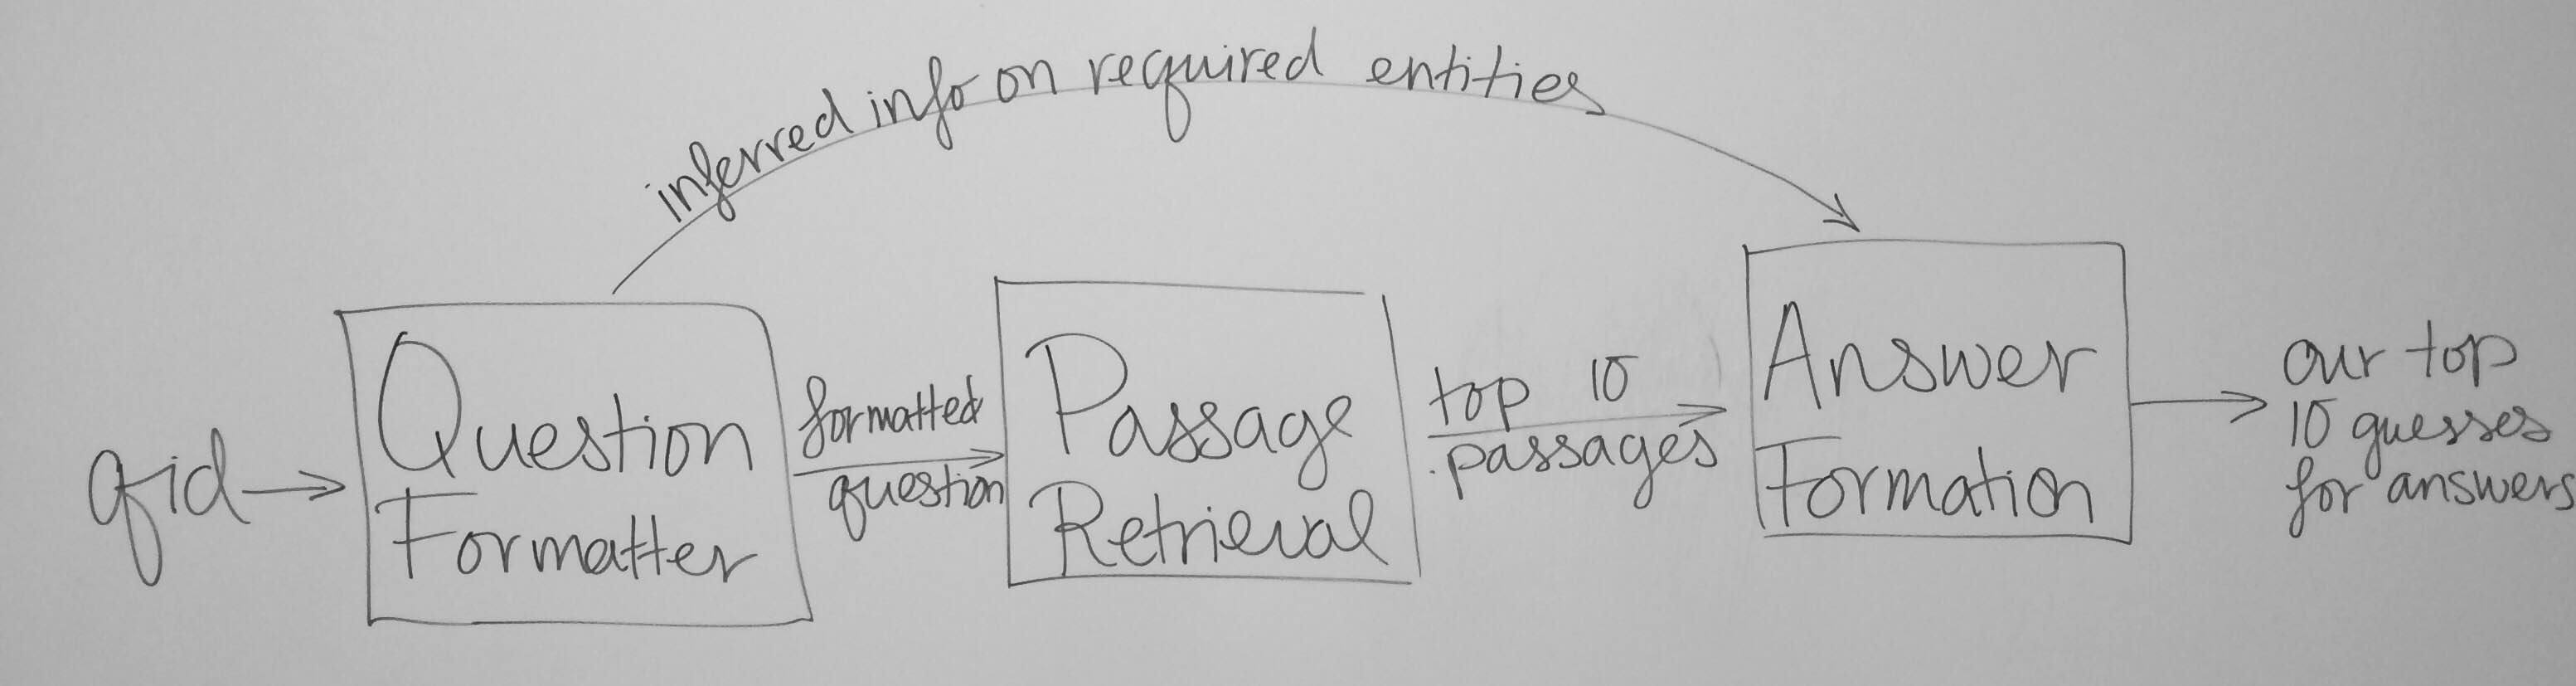
\includegraphics[width=1.0\textwidth]{images/diagram.jpg}
    \caption{Overview of our Question Answering system}
\end{figure}
At the very root of our QA system, we follow the description of the baseline system in the project writeup. We have three separate overall stages in our system, separated into three separate python classes:
\begin{enumerate}
\item Question Processing \texttt{question\_formatter.py}
\item Passage Retrieval \texttt{passage\_retrieval.py}
\item Answer Formation \texttt{answer\_formation.py}
\end{enumerate}

\subsection{Question Processing}
\begin{figure}[h]
    \centering
    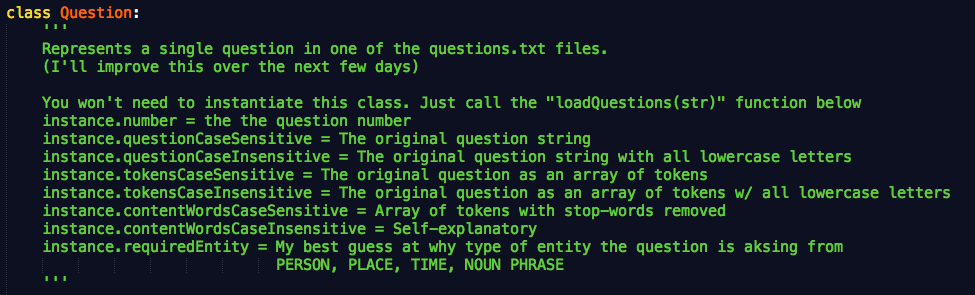
\includegraphics[width=1.0\textwidth]{images/question.png}
    \caption{Overview of the \texttt{Question} class.}
\end{figure}

This class provides our representation of the question that has been asked. The work we do in this step can be separated into two parts:
\begin{enumerate}
\item Basic question text processing
\item Making inferences about the nature of the question
\end{enumerate}

\subsubsection{Basic Question Text Processing}
We pull the text of the question from \texttt{questions.txt} and store its unique identifier, part of speech tags, and tokenized (both case-sensitive and case-insensitive) versions of the original text. All of this is done in the constructor of the \texttt{Question} class using the nltk library.

\subsubsection{Infer the Nature of the Question}
The work done in inferring the nature of the question is performed in the \texttt{Question} class, and the result is stored in the \texttt{descriptor} property of that class. The \texttt{descriptor} property on a \texttt{Question} instance is of type \texttt{Descriptor}, and stores the type of entity that we are looking for, along with some tokens in the tokenized question string that we believe are relevant.\\

We infer the nature of the question and its most relevant tokens by pattern matching. For example, upon inspecting the question files, we found that when the word \textit{"who"} appears in a question, we are most likely looking for a person in the answer. We found similar patterns for the words/phrases \textit{"where"},  \textit{"when"},  \textit{"how many"},  \textit{"how much"}, and  \textit{"what"}.\\

Given the appearance of those terms, we define the type of entity that is required in the answer (see the \texttt{REQUIREDENTITIES} map in the \texttt{Question} class).\\

Once we know the required type of entity, we attempt to infer relevant and descriptive tokens in the question for its required entity. Those inferences made are in the \texttt{get\textless Entity\textgreater Descriptor} functions in the \texttt{Question} class by pattern matching on the part-of-speech tags of the question.\\

\subsection{Passage Retrieval}
The overall interface of this step is as follows: we receive a question (of type \texttt{Question}, available in \texttt{question\_formatter.py}) and provide an instance of the \texttt{PassageRetrieval} class, which stores the most-similar passages for the top 10 documents in the \texttt{passages\_top\_10\_docs} property.
The steps taken during this step can be simplified as follows:
\begin{enumerate}
\item \textbf{Documents:} Process all the documents for a given question. In doing so, extract relevant text, identifiers, split into passages, etc.
\item \textbf{Term Frequency-Inverse Document Frequency:} Calculate the similarity between term frequency-inverse document frequency vectors between all passages and the question.
\item \textbf{Ranked Passages: }Return the top passages of the 
\end{enumerate}

Examining each of these more closely we have:\\
\subsubsection{Documents}
\begin{figure}[h]
    \centering
    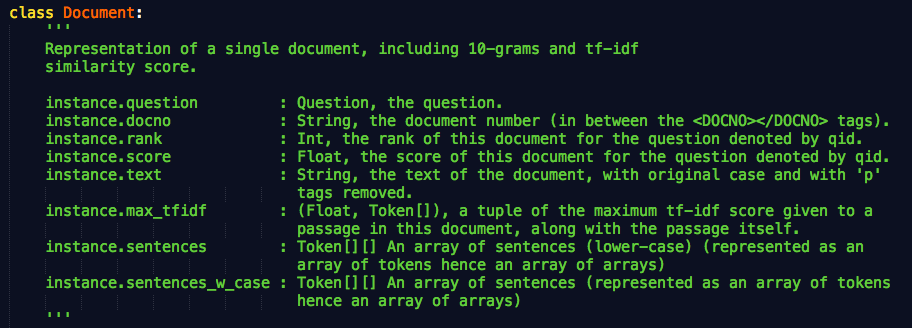
\includegraphics[width=1.0\textwidth]{images/document.png}
    \caption{Overview of the \texttt{Document} class.}
\end{figure}
\textit{Note: Processing the documents proved not to be as simple as we initially planned. The vast majority of the documents follow a similar markup structure, but a handful of them differed from the overall general structure. In those cases, we ignore the documents (don't include them in any of our subsequent system steps), as we found that those documents tend to be ranked low anyway.}\\

We begin processing the documents by pulling all of the text from the appropriate \texttt{top\_docs.$x$} file provided (with respect to dev or test) and separating it into entire documents, \texttt{qids} and all. Then, given the text of a document, we extract:
\begin{enumerate}
\item The \textit{rank} of the document.
\item The \textit{docno} (unique document identifier).
\item The relevancy \textit{score} of the document, as determined by the generator of the top\_docs documents.
\item The body (\textit{text}) of the document.
\item For the purpose of later calculations, we tokenize the document into sentences (\textit{sentences} and \textit{sentences\_w\_case}), and then those sentences into an array of tokens, with punctuation removed
\end{enumerate}

For the last extraction step, we remove punctuation because in a Question Answer system, the structure of the question is often different than the structure of the answer, so it would provide us little additional information. Also, we later use a tf-idf similarity measure so the punctuation may even hurt those calculations as certain punctuation doesn't occur frequently enough to be considered a stop word and would therefore have some effect on those final calculations.\\

Instead of defining a passage as a 10-gram, as is described in the baseline system, we define a passage as a sentence. Our justification for this is that the answer to a question is more likely to be contained in a sentence, as opposed to a sequence of 10 words, which might be spread over multiple sentences, including sentence fragments. This way, we were also able to simplify our Answer Formation step by knowing more of the general structure of the top-ranked passages that make it to that step.

\subsubsection{Tf-idf}
\begin{figure}[h]
    \centering
    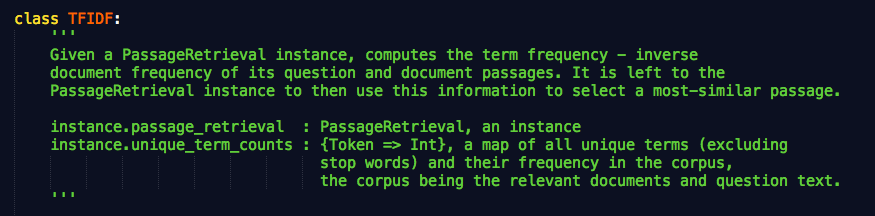
\includegraphics[width=1.0\textwidth]{images/tfidf.png}
    \caption{Overview of the \texttt{TFIDF} class.}
\end{figure}

\textit{Note: In this implementation of tf-idf calculation, we do not use vectors the length of the number of unique terms in the document. Instead, for each text fragment (i.e. question text or document passage), we only include the terms involved in that particular text fragment to avoid having massive arrays with a ton of 0 term frequencies. So in calculating the cosine similarity of two tf-idf vectors, we just infer count 0 for any terms that don't appear in both of the tf-idf vectors.}\\

We decided to create our own tf-idf class instead of using a library so that we had more flexibility in terms of our overall interface. In this class, we first calculate the total term frequency of each unique term in the corpus (all relevant documents and the question). We do this using Python's Counter class to simplify the number of loops we would normally have to use. After this, we calculate the tf-idf vector of the question. We calculate the tf-idf vector of the question first so that we only have to worry about storing that vector, and can then go on to compute the tf-idf vectors of each passage and immediately find the similarity score with the question, so that we can avoid having to store the tf-idf vectors of every passage as an intermediate step to eventually finding the cosine similarity. Doing this sped up our QA system.

\subsubsection{Top Ten Passages}
As we calculate tf-idf similarity scores between each passage in each document and the question, we keep track of only the top passage and its similarity score for each document for later calculations of what passage we should send to the Answer Formation step in our system.

After computing these scores, we examine the most-related passages of the top ten documents in our last major step in the system: the final ranking of the top passages. This is done in \textbf{Answer Formation}

\subsection{Answer Formation}
% TODO Sofo
\subsubsection{Top Passage}
This step has the largest impact on the final "top passages". Our rules are as follows:
\begin{itemize}
\item Initial ranking of each passage is the same of the ranking of its corresponding document in the top 10.
\item Length of the longest sequence of overlapping terms between passage and question:
	\begin{enumerate}
	\item If it is the lowest 5 documents, in terms of the length of the longest sequence of overlapping words between the passage and the question, it is moved to the bottom half (ranks 6-10) of the "top passages"
	\item Otherwise, it moves to the top half
	\end{enumerate}
\item The number of keywords that overlap. We examine the most relevant tokens from the question (as we discuss in Section \textbf{1.1: Question Processing}) and count the number of question keywords that also appear in each of the top passages.
\item We use a combination of the final two bullets to determine the document's final rank
\end{itemize}
\section{Performance Analysis}
% TODO Sofo

\section{Citations}
\subsection{Libraries}
\begin{itemize}
\item NumPy
\item NLTK
	\begin{itemize}
	\item POS-Tagger
	\item Sentence Tokenizer
	\item Word Tokenizer
	\end{itemize}
\item Python collections and difflib
\end{itemize}
\end{document}
